\documentclass{article}
\usepackage{graphicx} % Required for inserting images
\usepackage{amsmath}
\usepackage{geometry}
\usepackage{amssymb}
\usepackage{color}
\usepackage{CJKutf8}
\usepackage{float}
\usepackage{subfigure}
\usepackage{listings}
\usepackage{placeins}
\usepackage{enumitem}
\usepackage{booktabs}

\geometry{a4paper, scale=0.8}   
\linespread{2}
\definecolor{dark_green}{RGB}{0,102,51}
\title{Lab5 - Ethernet and ARP}
\author{Jiaxi Zhang}
\date{\today}
\begin{document}
\maketitle
\begin{CJK*}{UTF8}{gbsn}

\section{HTTP GET Packet}
The below four questions are based on the HTTP GET packet captured by Wireshark and
the screenshot is a printout of the packet.

\subsection{The 48-bit Ethernet address of my computer}
c6:19:77:e6:6b:1a
\subsection{The 48-bit Ethernet address of the destination}
00:00:5e:00:01:32. And this is not the MAC address of gaia.cs.umass.edu. 
It is a Virtual Router Redundancy Protocol address, which is used by my local router, and then forwards the request to gaia.
\begin{figure}[H]
    \centering
    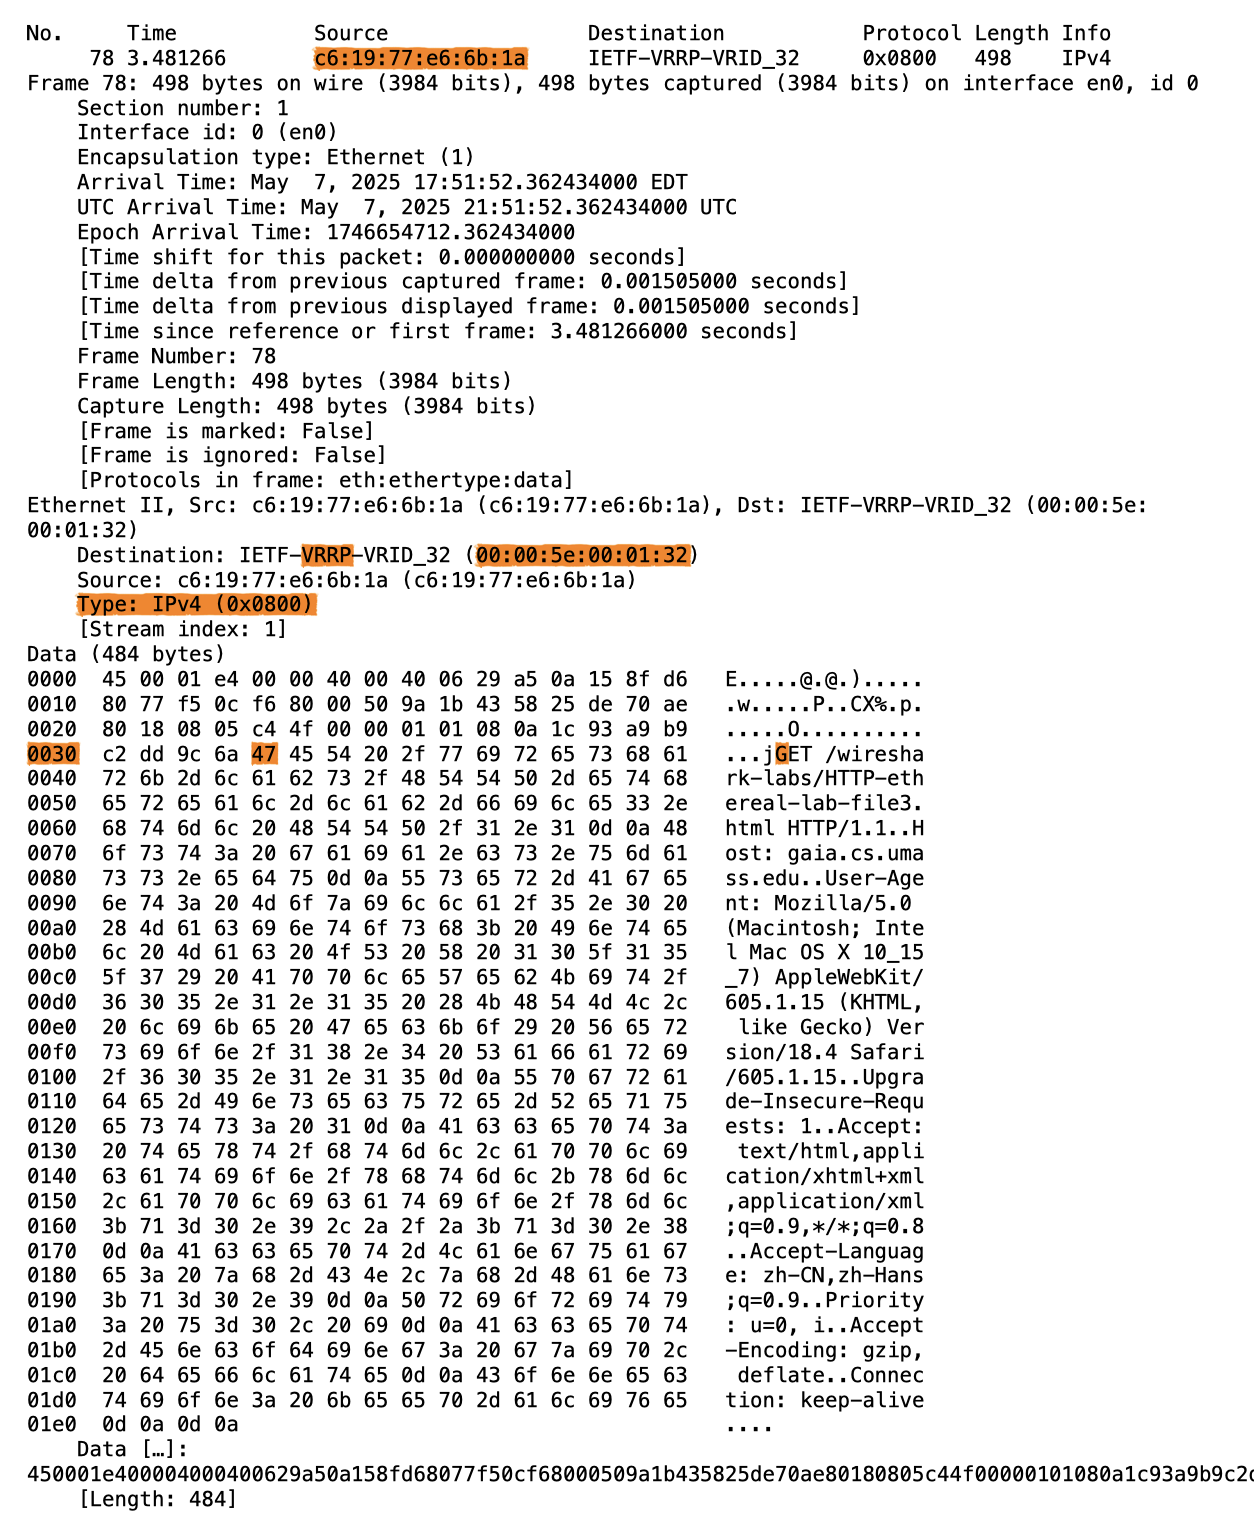
\includegraphics[width=0.8\textwidth]{1.png}
    \caption{Question1-4 Screenshot}
\end{figure}
\subsection{Hexadecimal value for the two-byte Frame type field}
0x0800. It indicates that the upper-layer protocol is IPv4.
\subsection{Byte Number}
The 'G' is the 53th byte from the very start of the Ethernet frame. We can find from the screenshot that
for each line, there are 16 bytes, and the line for 'G' appears starts from '0030', which is the 48th byte.
In the ASCII code, 'G' is 0x47, and we can find it in the 53rd byte with an offset of 52.


\section{HTTP 200 OK Packet}
The below four questions are based on the HTTP 200 OK packet captured by Wireshark and
the screenshot is a printout of the packet.
\begin{figure}[H]
    \centering
    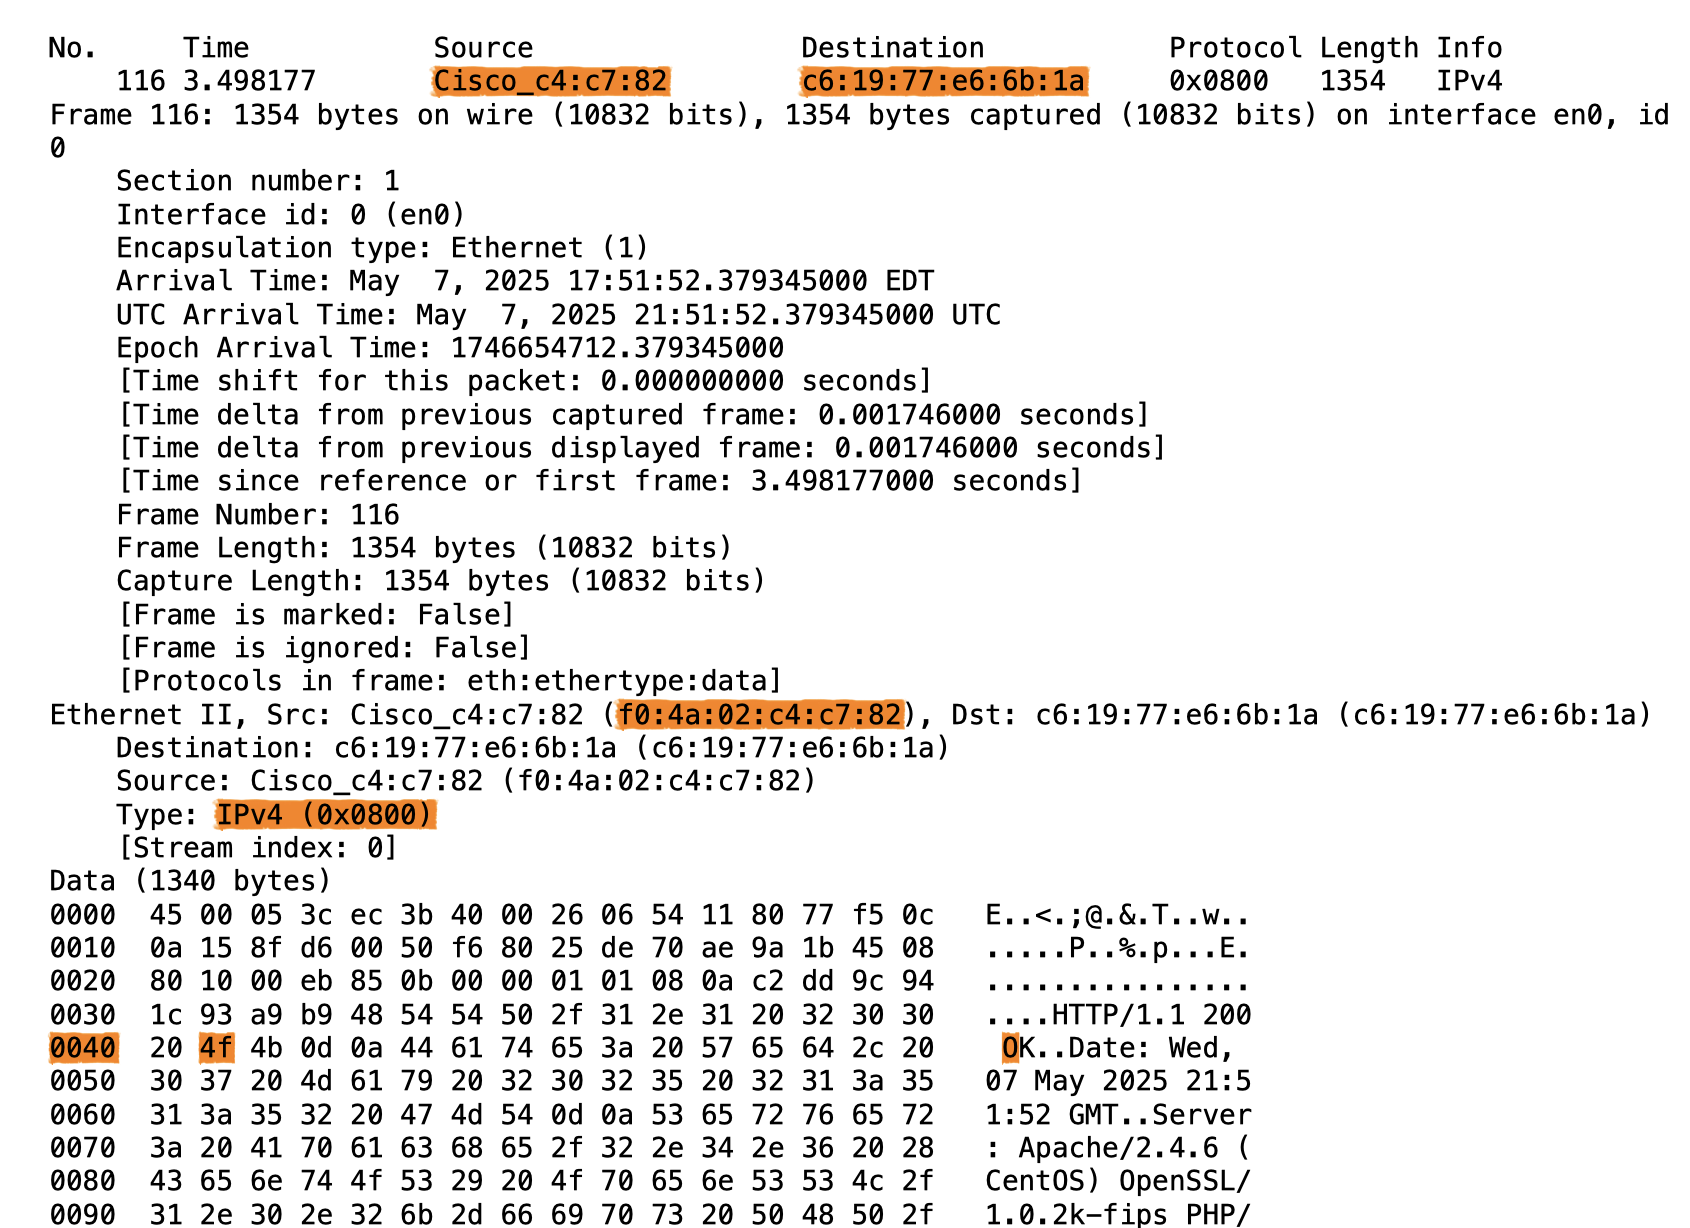
\includegraphics[width=0.8\textwidth]{2.png}
    \caption{Question5-8 Screenshot}
\end{figure}
\subsection{The 48-bit Ethernet address of source}
f0:4a:02:c4:c7:82. It is neither the MAC address of gaia.cs.umass.edu nor my computer.
But rather the default gateway or router (Cisco device in this situation) that forwarded the response from gaia.cs.umass.edu.
\subsection{The 48-bit Ethernet address of destination}
c6:19:77:e6:6b:1a. It is the MAC address of my computer.
\subsection{Hexadecimal value for the two-byte Frame type field}
0x0800. It indicates that the upper-layer protocol is IPv4.
\subsection{Byte Number}
The 'O' is the 66th byte from the very start of the Ethernet frame. We can find from the screenshot that
for each line, there are 16 bytes, and the line for 'O' appears starts from '0040', which is the 64th byte.
In the ASCII code, 'O' is 0x4F, and we can find it in the 66th byte with an offset of 65.

\section{ARP cache}
\subsection{Contents of ARP Cache}
Below is the output of the \texttt{arp -a} command on my computer, which displays the current contents of the ARP cache:

\begin{lstlisting}
    arp -a

    1536-gw.net.nyu.edu (10.21.128.1) at 0:0:5e:0:1:32 on en0 ifscope [ethernet]
    10-21-143-214.dynapool.wireless.nyu.edu (10.21.143.214) at c6:19:77:e6:6b:1a on en0 
        ifscope permanent [ethernet]
    1536-bcast.net.nyu.edu (10.21.255.255) at ff:ff:ff:ff:ff:ff on en0 ifscope [ethernet]
    ? (169.254.169.254) at f0:4a:2:c4:b9:c2 on en0 [ethernet]
    mdns.mcast.net (224.0.0.251) at 1:0:5e:0:0:fb on en0 ifscope permanent [ethernet]
    ? (239.255.255.250) at 1:0:5e:7f:ff:fa on en0 ifscope permanent [ethernet]
\end{lstlisting}

\subsection*{Meaning of Each Column}
\begin{itemize}
  \item \textbf{Hostname}: If resolvable, this is the DNS name associated with the IP address (eg \texttt{1536-gw.net.nyu.edu}).
  \item \textbf{IP Address}: The IP address for which the ARP entry maps a MAC address(eg. \texttt{10.21.128.1})
  \item \textbf{MAC Address}: The Ethernet hardware address (e.g., \texttt{00:00:5e:0:1:32}).
  \item \textbf{Interface}: The network interface through which the ARP entry applies (in this case, \texttt{en0}).
  \item \textbf{Flags}: Includes whether the entry is dynamically learned or permanent, and the link layer type, which is typically \texttt{[ethernet]}.
\end{itemize}

\section{Observe ARP In Action}
I tried http://gaia.cs.umass.edu/wireshark-labs/HTTP-wireshark-lab-file3.html
which is instructed in the lab manual. However, even though with all the caches cleared, I still
cannot observe the ARP packets in the Wireshark capture.
So I choose to use the given file in the lab manual for the following questions.

\subsection{Request}
\begin{figure}[H]
    \centering
    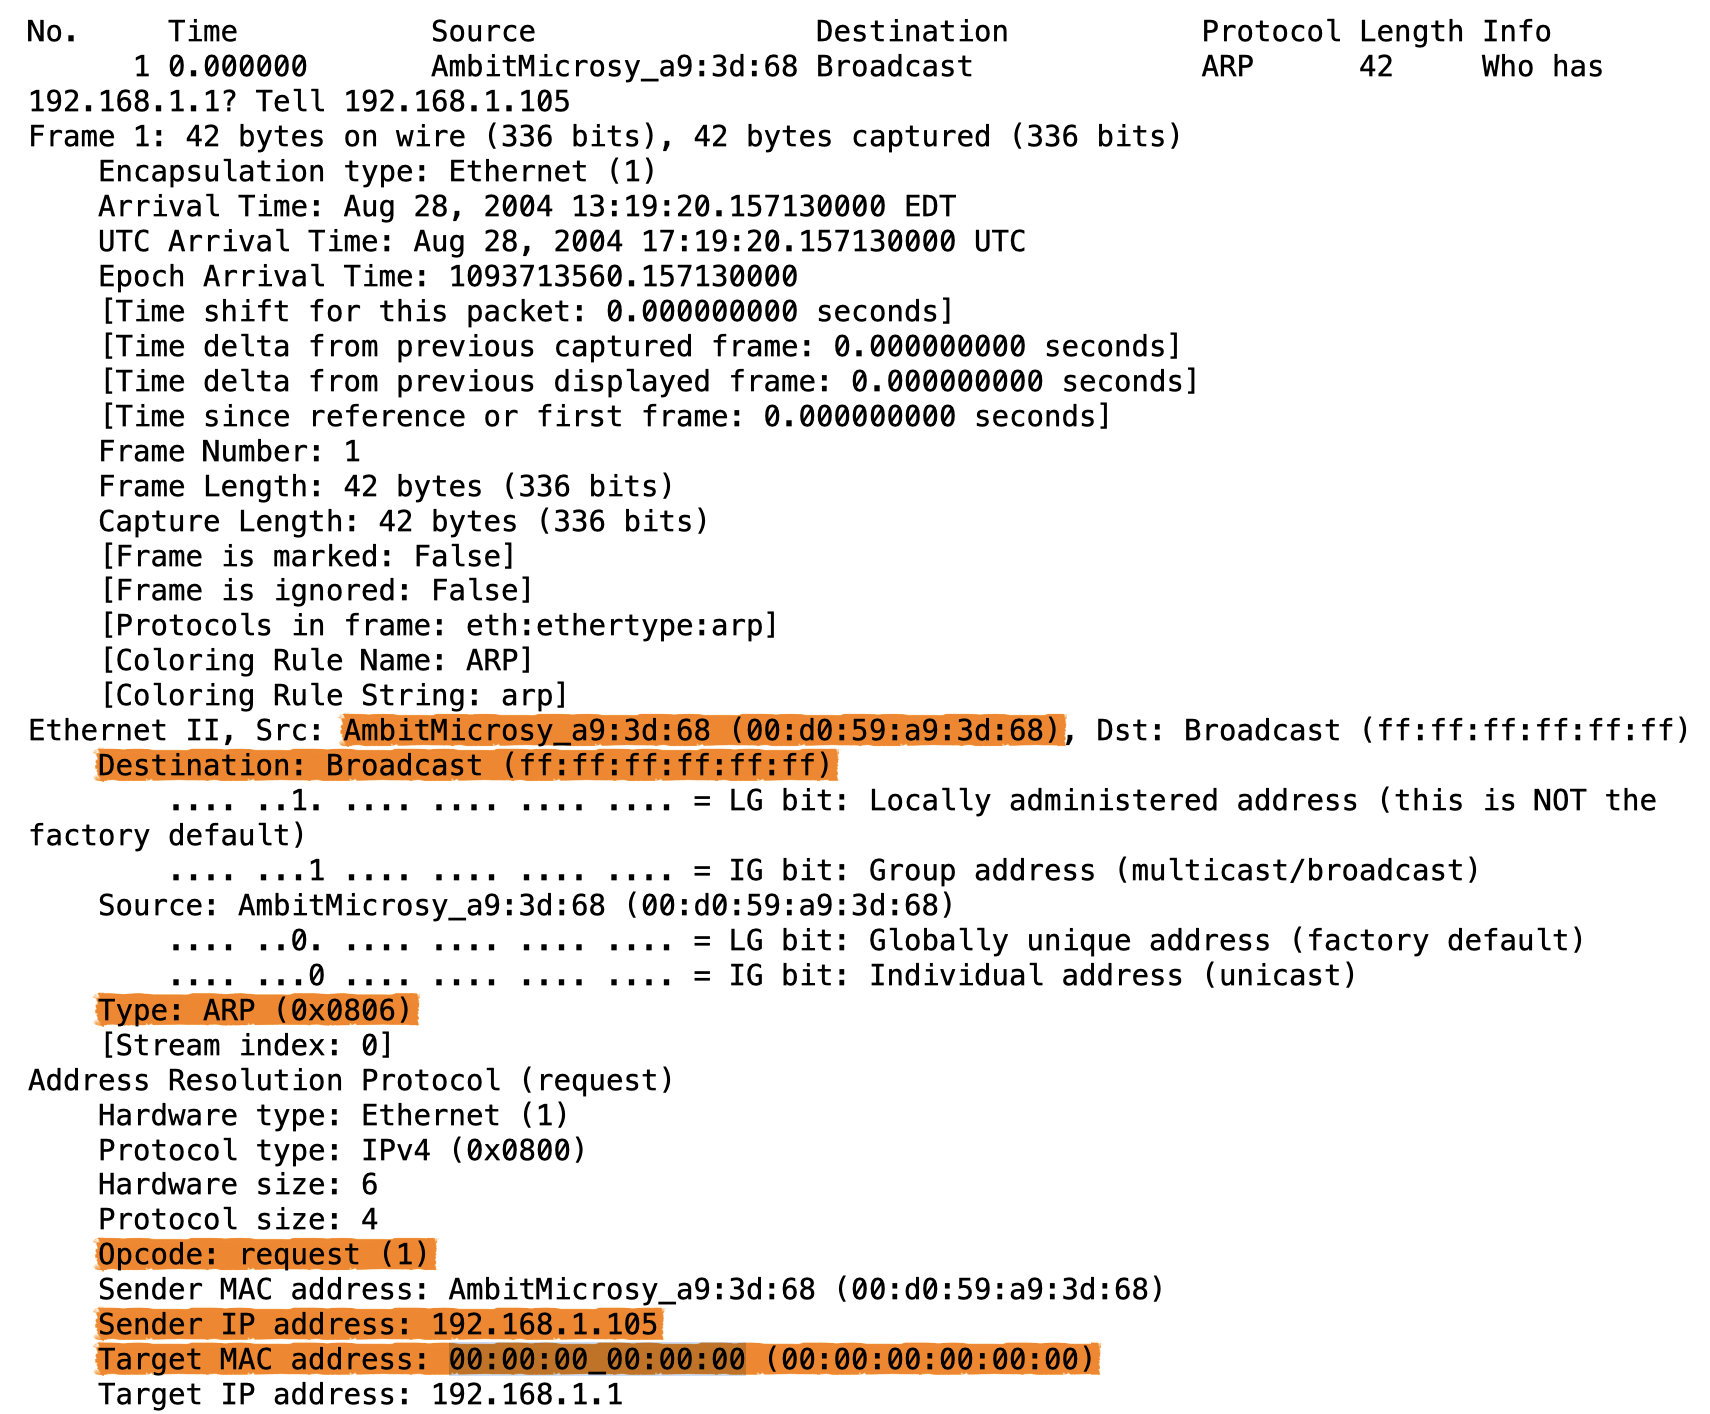
\includegraphics[width=0.8\textwidth]{12.png}
    \caption{Question5-8 Screenshot}
\end{figure}
\subsection{Hexadecimal values for the source and destination addresses}
In the first ARP packet containing ARP Request,
Source MAC: 00:d0:59:a9:3d:68, and Destination MAC: ff:ff:ff:ff:ff:ff
\subsection{Frame type field and upper-layer protocol}
Type: 0x0806, 
Upper-layer protocol: ARP


\subsubsection{How many bytes from the very beginning of the Ethernet frame does the ARP opcode field begin?}
According to the RFC 826,
the ARP opcode field is located at byte 21 in the ARP packet because
there are 14 bytes of Ethernet header and 6 bytes of ARP header before the opcode field.
\subsubsection{the value of the opcode field}
The value of the opcode field is 1. We can find
in the screenshot that "Opcode: request (1)"
\subsubsection{whether containing the sender's IP address}
Yes, it contains the sender's IP address. We can find
in the screenshot that "Sender IP address: 192.168.1.105"
\subsubsection{Where in the ARP request does the “question” appear?}
The "question" appears in the "Target MAC address" field.
Since the sender does not know the MAC address of the target, it is set to 00:00:00:00:00:00.

\subsection{Response}
\begin{figure}[H]
    \centering
    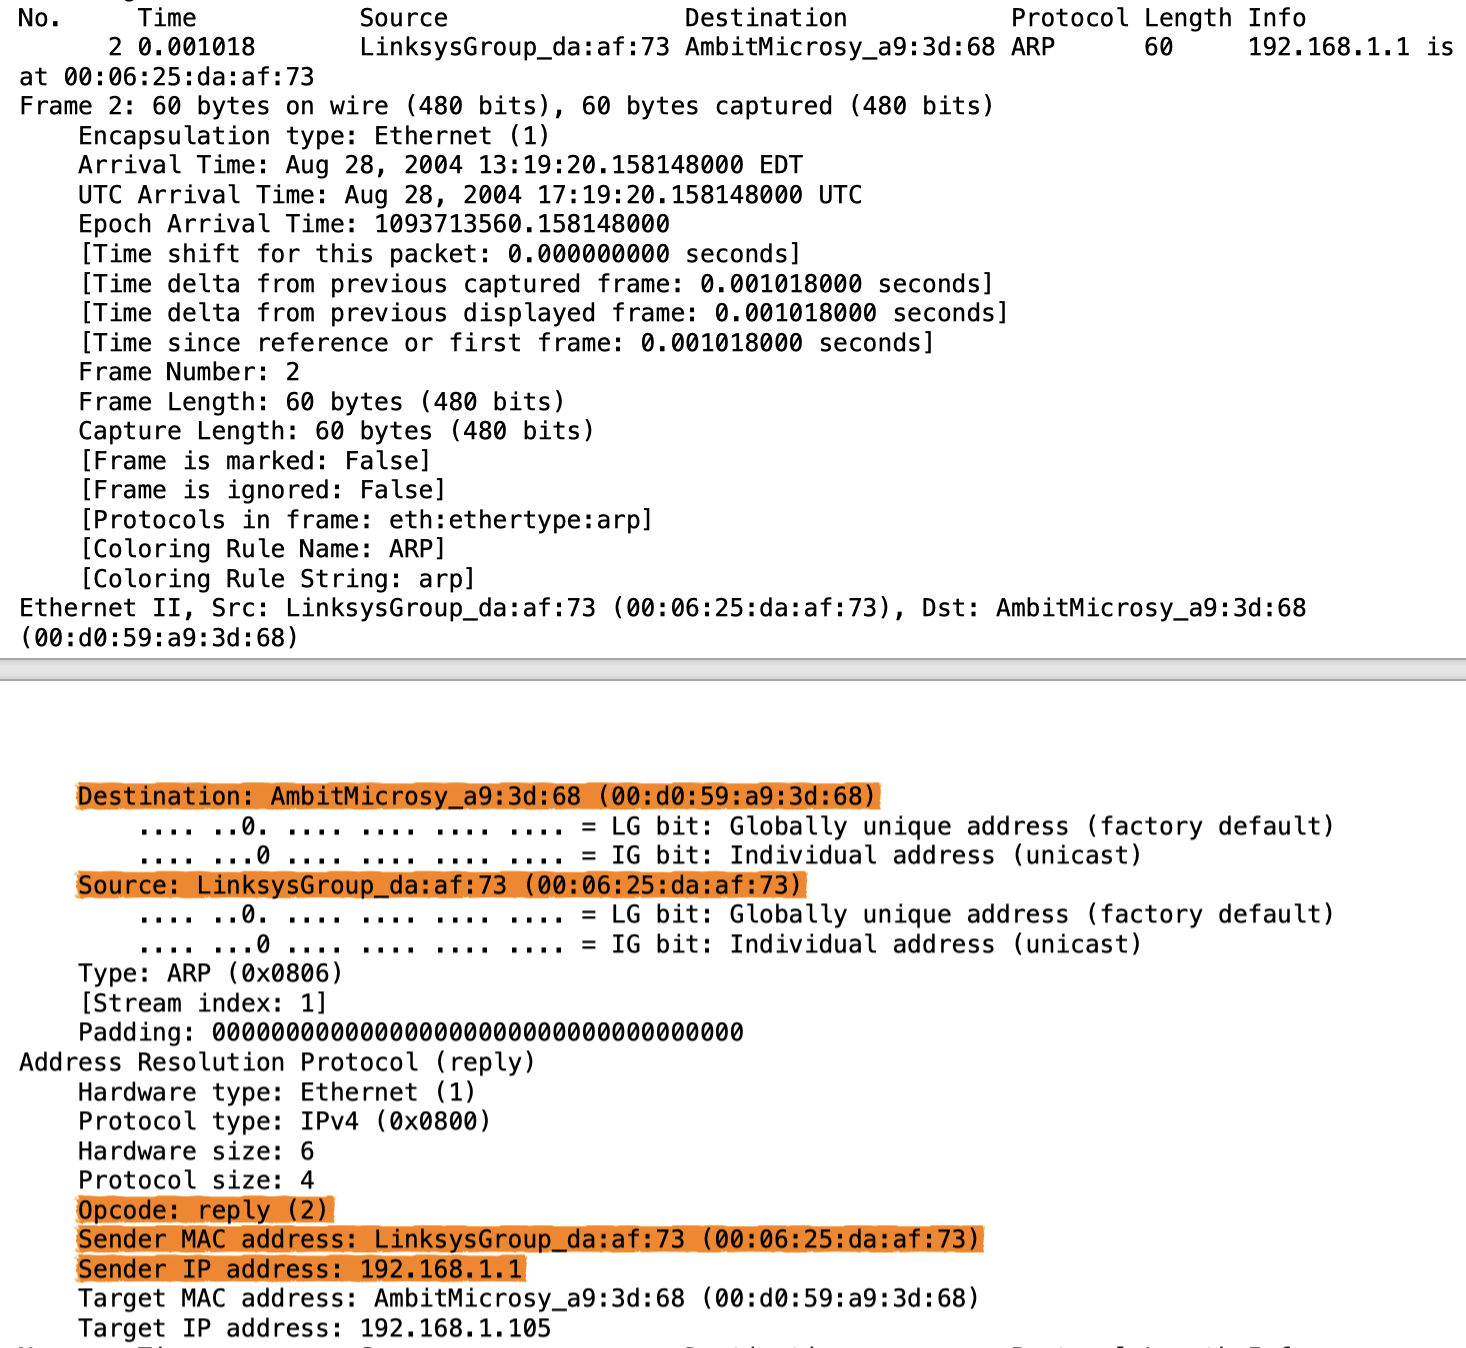
\includegraphics[width=0.8\textwidth]{14.png}
    \caption{Question5-8 Screenshot}
\end{figure}
\subsubsection{How many bytes from the very beginning of the Ethernet frame does the ARP opcode field begin?}
According to the RFC 826,
the ARP opcode field is located at byte 21 in the ARP packet. The same as the ARP request.
\subsubsection{the value of the opcode field}
The value of the opcode field is 2. We can find
in the screenshot that "Opcode: reply (2)"
\subsubsection{Where in the ARP message does the “answer” to the earlier ARP request appear?}
The "answer" appears in the "Sender MAC address" field and "Sender IP address" field.
Sender MAC address: LinksysGroup\_da:af:73 (00:06:25:da:af:73) Sender IP address: 192.168.1.1
\begin{figure}[H]
    \centering
    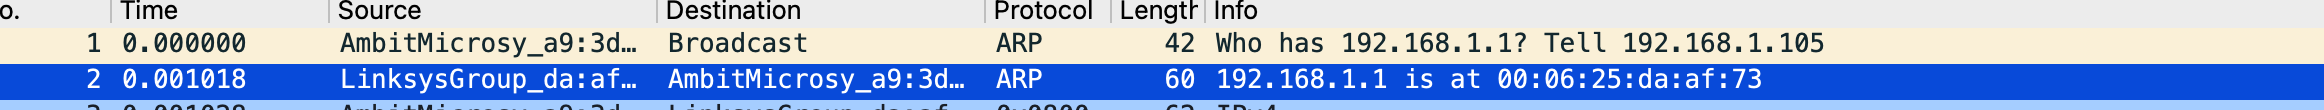
\includegraphics[width=0.8\textwidth]{13.png}
    \caption{Question5-8 Screenshot}
\end{figure}
\subsection{Hexadecimal values for the source and destination addresses}
Destination: AmbitMicrosy\_a9:3d:68 (00:d0:59:a9:3d:68)\
Source: LinksysGroup\_da:af:73 (00:06:25:da:af:73)

\subsection{The reason for not getting the ARP response}
There is no ARP reply to the request in packet 6 
because the host with IP address 192.168.1.117 might be either not active on the network at the time, or was configured not to respond to ARP requests. 


\section{Extra Credit}
\subsection{}
If I entered the correct IP address, but the wrong Ethernet address for that remote interface when manually adding an entry,
the ARP cache would not be able to resolve the IP address to the correct MAC address. It will be successful in adding the entry to the ARP cache, 
but the entry will not be useful for communication and the target host will not be reachable.
\end{CJK*}
\end{document}
